\subsubsection{Cosmological I-front propagation}
\label{sec.tests.fld}

This test problem examines Enzo's flux-limited diffusion radiation
transport and associated ionization chemistry solvers on a
cosmological I-front test.  This corresponds to test problem 4.6 from
\cite{ReynoldsHayesPaschosNorman2009}, run using the cosmological
deceleration parameter $q_0 = 0.05$ and initial redshift $z_i=10$.
Here, the physics of interest is the expansion of a \ion{H}{2} region
in a uniform gas around a single monochromatic ionizing source (with
frequency $h\nu = 13.6$ eV).  In this problem the I-front propagates
rapidly at first, approaching 90\% of the Str{\" o}mgren radius by a
scaled redshift of $-\log\left[(1+z)/(1+z_i)\right] \approx 0.15$,
before cosmological expansion overtakes ionization, pushing the Str{\"
o}mgren radius outward faster than the I-front can propagate.  Here,
the Str{\" o}mgren radius is analytically given by
\[
   r_S(t) = \left[\frac{3\dot{N}_{\gamma}}{4\pi \alpha_{\rm B}
   n_{\rm H}(t)^2}\right]^{1/3}, 
\]
where $\dot{N}_{\gamma} = 5 \times 10^{48}$ photon sec$^{-1}$ is the
stength of the ionizing source, $\alpha_{\rm B} = 2.52 \times 10^{-13}$
s$^{-1}$ is the \ion{H}{2} recombination rate, and $n_H(t)$ is the
proper number density of hydrogen.  We then define $\lambda =
\alpha_{\rm B}\, n_{H,i}\, /\, H_0\, / (1+z_i)$, where the subscript $i$
indicates the quantity at the initial redshift.  The analytical
solution for the I-front position as a function of time (or actually
of the time/redshift-dependent expansion coefficient $a(t)$) is then

\begin{eqnarray*}
   r_I(t) &=& r_{S,i} \left[\lambda e^{-\tau(a)} \int_1^{a(t)}
     e^{\tau(\tilde a)} \left(1 - 2q_0
     + \frac{2q_0(1+z_i)}{\tilde{a}}\right)^{-1/2}\mathrm
     d\tilde{a}\right]^{1/3}, \quad\text{where} \\ 
   \tau(a) &=& \lambda\frac{6q_0^2(1+z_i)^2}{F(a)-F(1)}, 
     \quad\text{and} \\
   F(a) &=& \left[2-4q_0 - \frac{2q_o(1+z_i)}{a}\right] 
      \left[1-2q_0 + \frac{2q_0(1+z_i)}{a}\right]^{1/2}.
\end{eqnarray*}

The simulation parameters are a box size $L_i\approx 27$ kpc, Hubble
constant $H_0 = 1$ (in units of 100 km/s/Mpc), and cosmological
constants $\Omega_m = 0.1$, $\Omega_A=0$ and $\Omega_b = 0.1$.  The
initial values for the simulation are a radiation energy density
$E_{r,i} = 10^{-35}$ erg cm$^{-3}$, temperature $T_i = 10^4$ K,
density $\rho_{b,i} = 2.35 \times 10^{-28}$ g cm$^{-3}$, and an
ionized hydrogen fraction $n_{\rm HII}/n_{\rm H} = 0$.

In Figure \ref{fig.fld}, we plot profiles of the \ion{H}{1} and
\ion{H}{2} fractions at the redshifts $z=\{6.24,\, 2.29,\, 1.02\}$, as
well as the ratio of the I-front and Str{\" o}mgren radii throughout
the simulation.  As seen in the left panel (species fractions as a
function of radius), the I-front is initially quite narrow, but slowly
becomes wider as the simulation proceeds due to the diffusion
approximation used by the radiative transfer scheme.  However, as seen
in the I-front propagation history plot (right panel), the computed
I-front location very accurately matches the exact value.

\begin{figure}
\begin{center}
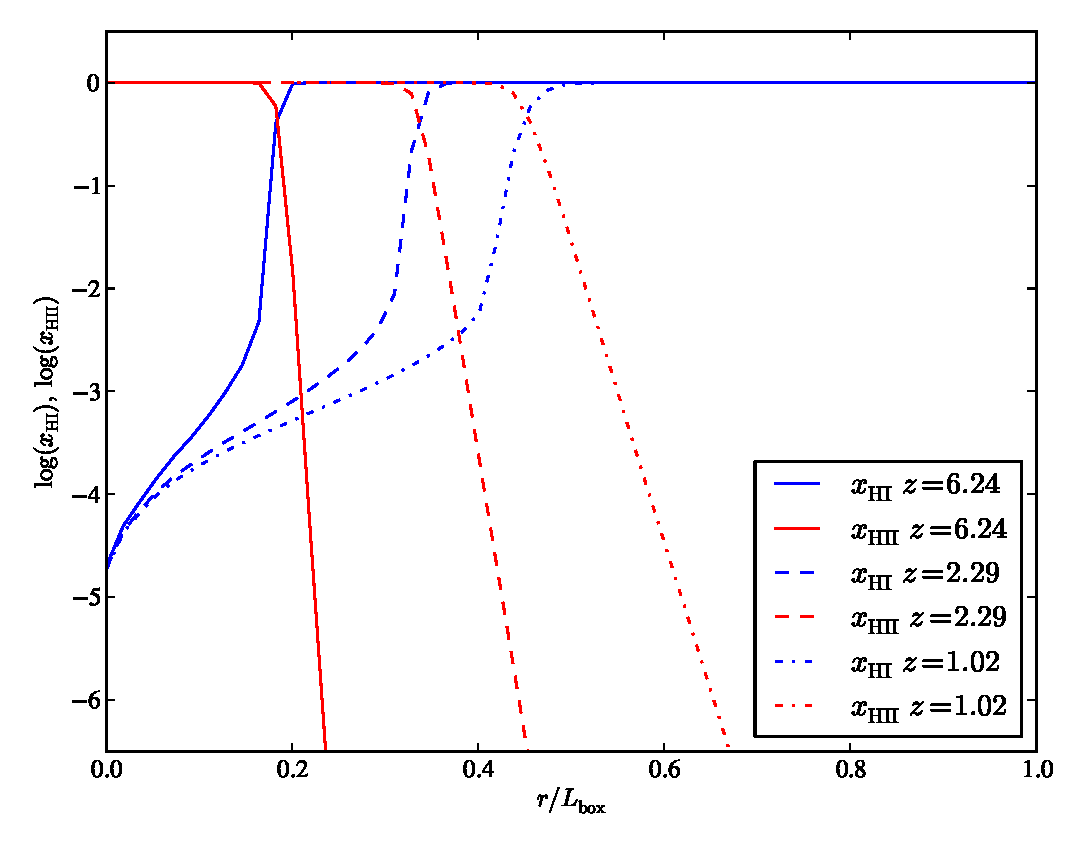
\includegraphics[width=0.45\textwidth]{figures/FLDprofiles.eps}
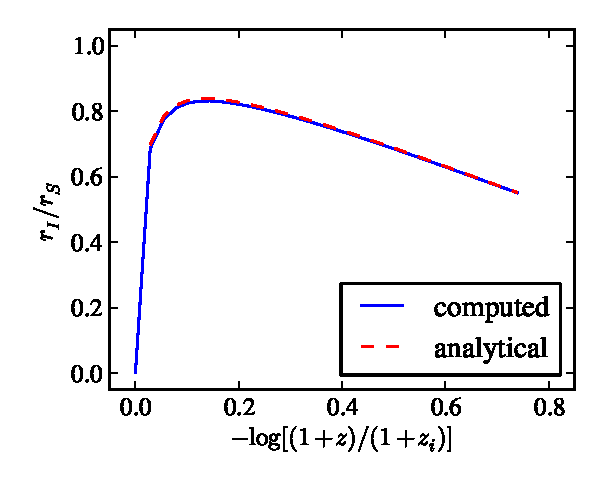
\includegraphics[width=0.45\textwidth]{figures/FLDhistory.eps}
\caption{Ionized fraction profiles and I-front location history for
the propagation of an ionization front in an expanding universe, using
\enzo's flux-limited diffusion radiation transport method.  Left
panel: profiles of the \ion{H}{1} and \ion{H}{2} fractions (blue and
red lines, respectively) at redshifts $z=\{6.24,\, 2.29,\, 1.02\}$
(solid, dashed, dot-dashed lines).  Right panel: ratio of the I-front
and Str{\" o}mgren radii as a function of scaled redshift in the test
problem (blue solid line) and analytical solution (red dashed line).}
\label{fig.fld}
\end{center}
\end{figure}

%%% Local Variables: 
%%% mode: latex
%%% TeX-master: "ms"
%%% End: 
